\documentclass[12pt]{article}

\usepackage{sbc-template}
\usepackage{graphicx,url}
\usepackage[utf8]{inputenc}
\usepackage[brazil]{babel}
\usepackage[latin1]{inputenc}  
\usepackage{xcolor}

\sloppy

\title{Comparando Flutter com React-Native para a Criação de Aplicativo Móveis Híbridos: O Caso da App Melhores Marcas}

\author{Marcos Antônio Maia Sampaio Júnior\inst{1}, Luis Paulo da Silva Carvalho\inst{1}}

\address{Instituto Federal da Bahia (IFBA)\\
  Av. Sérgio Vieira de Melo, 3150 - Zabelê\\  
  Vitória da Conquista, Bahia, Brasil\\ 
  \email{marcos.amsj45@gmail.com, luiscarvalho@ifba.edu.br}
}

\begin{document} 

\maketitle

\begin{abstract}
This work proposes a comparison between Flutter and React-Native, using a version of the "Best Brands" application in both \textit{frameworks}. The app is a didactic one and originally created in React-Native, serving as a proof of concept in Mobile Programming classes of the "Bacharelado em Sistemas de Informação", a graduation course held in IFBA, Vitória da Conquista. The article presents theoretical and technological foundations, detailing React-Native and Flutter. The description of the "Best Brands" application is highlighted, featuring a \textit{feed} screen with a \textit{lazy-loading} mechanism. We developed the Flutter version of the app during the course of the work, aiming to faithfully replicate the original React-Native version. The comparative evaluation between the two \textit{frameworks} included the use of a metric regarding the interval time required during its boot-up and the benefits of IDE integration (VSCode).
\end{abstract}
     
\begin{resumo} 
Esse trabalho propõe uma comparação entre Flutter e React-Native, utilizando uma versão do aplicativo "Melhores Marcas" em ambos os \textit{frameworks}. O app é didático e originalmente criado em React-Native, sendo utilizado como prova de conceito em aulas de Programação Móvel do curso de Bacharelado em Sistemas de Informação do IFBA, campus Vitória da Conquista. O artigo apresenta fundamentos teóricos e tecnológicos, detalhando o React-Native e o Flutter. Destaca-se a descrição da aplicação "Melhores Marcas", que possui uma tela de \textit{feed} com mecanismo de \textit{lazy-loading}. A versão Flutter do app foi desenvolvida durante a realização do trabalho, buscando replicar fielmente a versão original em React-Native. A avaliação comparativa entre os dois \textit{frameworks} inclui um estudo sobre uma métrica de inicialização/uso do aplicativo e integração com a IDE de desenvolvimento, VSCode.
\end{resumo}

\section{Introdução}
Os dispositivos móveis vêm se tornando cada vez mais presentes no nosso dia a dia. Em 2021, 84,4\% dos brasileiros acima dos 10 anos de idade já possuíam um aparelho para uso próprio \cite{ref_2}. Eles deixaram de ser apenas uma “caixinha” que usamos para realizar ligações e ganharam diversos novos usos com o avanço tecnológico, sendo utilizados para fins de entretenimento através de redes sociais e jogos, busca de informação por meio de acesso a notícias, comunicação mais simples através de aplicativos como o WhatsApp, além de serem utilizados como ferramentas de trabalho.

Com toda essa popularidade, empresas viraram sua atenção para o mercado de desenvolvimento mobile. Em 2021 a demanda por programadores da área aumentou em 600\% \cite{ref_3}, o que revela que a indústria de \textit{software} busca alavancar investimentos e lucros nesta área através de aplicativos que servem como plataformas para oferecerem serviços, tais como, por exemplo, plataformas de streaming e bancos online. Há casos onde a própria aplicação é o produto sendo oferecido, tais como jogos e redes sociais ou apps com um nicho específico, aplicações para a prática de exercícios físicos ou aplicações para marcar encontros. 

Programação móvel, sendo uma área do desenvolvimento de \textit{software} com bastante visibilidade, apresenta desafios para quem quer ingressar nela, pois é uma ramificação mais recente e que está em constante evolução. Por exemplo, existem diversas plataformas e \textit{frameworks} que podem ser utilizados para o desenvolvimento de apps. Os mais populares atualmente são o React-Native e o Flutter, a primeira sendo utilizada por 32\% dos desenvolvedores da área e a segunda por 46\%, dados do ano de 2022 \cite{ref_1}. 

O React-Native (mais detalhes na Seção \ref{sec:R-N}) surgiu através da necessidade da equipe do Facebook de publicar uma nova versão do aplicativo de sua rede, já que o primeiro criado utilizando HTML5 apresentava problemas de desempenho e estabilidade. O próprio Zuckerberg comentou em 2012 que seu maior erro foi apostar demais no HTML5 \cite{ref_5}. A partir disso, alguns funcionários do Facebook se reuniram em uma Hackathon para desenvolver um \textit{framework} para desenvolvimento mobile utilizando JavaScript. Em março de 2015 seria lançado o React-Native com suporte para iOS e em setembro do mesmo ano seria lançada sua versão para Android. 

O Flutter (mais detalhes na Seção \ref{sec:Flutter})  é um \textit{framework} desenvolvido pela Google, que surgiu em suas primeiras versões em 2015 com o nome de "Sky". Inicialmente funcionava apenas para Android. Em 2018 o Flutter teve o lançamento de sua versão 1.0, já com suporte para iOS e sendo considerada sua versão estável e pronta para produção.
 
Decidir qual desses \textit{frameworks} utilizar para criar aplicativos é importante para os programadores e empresas. Então é necessário que todos estejam atentos aos pontos positivos e negativos que cada um deles apresenta. Diante deste desafio, este trabalho busca apresentar uma comparação entre Flutter e React-Native. 
 
Para atingir o objetivo foi criada uma versão do app Melhores Marcas. Melhores Marcas é um app didático criado em React-Native e é usado nas aulas da disciplina de Programação Móvel do curso de Bacharelado em Sistemas de Informação do IFBA, campus Vitória da Conquista, como uma prova de conceito dos conteúdos da disciplina. A nova versão foi feita com Flutter, buscando aproximar o produto final da aplicação original. Com as duas versões em mãos, foram realizadas comparações, tais como, desempenho, facilidades de uso dos \textit{frameworks} e outras.

\section{Trabalhos Relacionados} \label{sec:Relacionados}
Nesta seção, são analisados trabalhos correlatos, que realizaram algum esforço sistemático comporativo entre os dois \textit{frameworks} alvos, React-Native e Flutter.

No trabalho \cite{ref_10}, os autores realizam um estudo com o Flutter através do qual apresentam a arquitetura do \textit{framework}, o funcionamento de sua interface e as ferramentas utilizadas em conjunto para o desenvolvimento de aplicações Flutter. Citam desde a instalação do Flutter até o caso do app que utilizaram como estudo de caso. Por fim, realizam uma breve comparação com o React-Native, analisando as diferenças entre as sintaxes dos \textit{frameworks}.

Em \cite{ref_6}, Wenhao Wu compara os 2 \textit{frameworks} no desenvolvimento de aplicações móveis. O autor faz uma comparação bem parecida com a realizada neste trabalho, recriando um app que tem uma versão original criada utilizando React-Native. No seu trabalho, Wu realiza algumas comparações, sendo elas, navegação entre telas, modularização de componentes, estilização e desempenho do aplicativo.

Em \cite{ref_7} Jakub Jagiello realiza também comparações entre os desempenhos dos \textit{frameworks} utilizando duas aplicações. Os testes que o autor realiza buscam encontrar a quantidade de quadros perdidos durante a execução e o tempo que leva para renderizar o app. Ele também se preocupa em realizar os testes com o Flutter duas vezes, uma em modo de debug (depuração) e outra em \textit{release} (produto final em situação de entrega).

O trabalho \cite{ref_9}, realizado por Breno Coll de Freitas, é mais extenso, abordando primeiramente os dois \textit{frameworks}, suas arquiteturas e seus processos de renderização. No estudo de caso realizado são utilizadas 5 aplicações diferentes. As duas primeiras são parecidas com as utilizadas em \cite{ref_7}. São dois apps que funcionam como cronômetros, o primeiro sendo um cronômetro único e o segundo apresenta seis cronômetros. O terceiro aplicativo é um contador de toques na tela, que é a aplicação padrão gerada pelo Flutter quando se inicia um novo projeto. O quarto app é um tela com 2 botões, onde cada um leva para uma tela diferente e essas novas telas apresentam apenas a opção de retornar a tela anterior. Tal aplicação tem como objetivo testar a navegação entre telas em cada \textit{framework}. A última aplicação apresenta uma lista com mil itens, e tem como propósito avaliar o desempenho de cada \textit{framework} ao lidar com listas extensas.

Em \cite{ref_8}, os autores realizam uma comparação entre os dois \textit{frameworks} com foco na produtividade, esse comparativo se deu a partir da construção de duas aplicações iguais, cada uma utilizando um dos \textit{frameworks}. Os autores definiram alguns critérios para realizar essa comparação: instalação do \textit{framework}, emulação da aplicação (uso de emuladores), consumo de API, estilização de interface, documentação, conteúdos Online, dependências externas, estabilidade de atualizações, build do aplicativo, pontos positivos e negativos. 

Como pode ser percebido ao longo desta seção, a preocupação de se comparar os dois \textit{frameworks} mais utilizados atualmente na indústria de desenvolvimento de aplicativos existe. Embora este trabalho aqui apresentado replique muitos objetivos e métodos usados anteriormente, ele se distancia dos outros pelas contribuições (mais detalhes na Seção \ref{sec:contribuicoes}): (1) o código-fonte está sendo disponibilizado e (2) o material está sendo usado em disciplina do curso de Bacharelado de Sistemas de Informação (BSI) do IFBA, campus Vitória da Conquista, para habilitar estudantes no desenvolvimento de aplicativos Flutter.

\section{Fundamentos Teóricos e Tecnológicos} \label{sec:FTT}

Nesta Seção são apresentados alguns conceitos e usos práticos relacionados ao uso do Flutter e React-Native.

\subsection{React-Native} \label{sec:R-N}

React Native é um \textit{framework} de desenvolvimento de aplicativos móveis que permite aos desenvolvedores criar aplicativos para iOS e Android usando JavaScript e React. O React Native funciona de maneira semelhante ao React para a Web, com a diferença de que ele renderiza componentes móveis nativos (do iOS e do Android) em vez de elementos HTML. 

Para que o React Native funcione corretamente, é necessário ter instalado em seu ambiente de desenvolvimento as seguintes ferramentas e \textit{frameworks}: 

\begin{enumerate}
    \item \textbf{Node.js}: uma plataforma de desenvolvimento que permite aos desenvolvedores executar código JavaScript fora de um navegador; 
    \item \textbf{Yarn ou NPM}: gerenciadores de pacotes que permitem a instalação e gerenciamento de bibliotecas e dependências de projetos javascript; 
    \item \textbf{React-Native CLI}: a interface de linha de comando que cria e gerencia projetos do React-Native;
    \item \textbf{NPX}: executável que faz parte do Node.js e é usado para executar pacotes Node.js sem precisar instalá-los globalmente no sistema operacional. 
\end{enumerate}

Além dessas ferramentas, é preciso instalar algumas dependências específicas do React Native, como o próprio sdk React Native e o Metro Bundler, que é o servidor de desenvolvimento que permite carregar o código JavaScript no dispositivo ou em um emulador.


\subsection{Flutter} \label{sec:Flutter}

Flutter é um \textit{framework} de desenvolvimento de aplicativos móveis criado pelo Google. Ele permite que os desenvolvedores criem aplicativos nativos para iOS, Android, web e desktop a partir de uma única base de código, escrita na linguagem de programação Dart. 

O funcionamento desse \textit{framework} depende do Flutter SDK, que é um kit de ferramentas que contém o que é necessário para criar aplicativos móveis nativos. Inclui o Dart SDK, o Flutter engine, um conjunto de widgets, ferramentas de linha de comando e plugins. Cada um destes elementos são explicados nos próximos parágrafos.

O Dart SDK é uma linguagem de programação orientada a objetos desenvolvida pela Google, que é usada para escrever aplicativos Flutter. Ele inclui um compilador Dart, uma máquina virtual Dart e uma biblioteca padrão que fornece muitas funcionalidades comuns de programação. 

Os widgets são componentes de que podem ser combinados para formar a interface completa do usuário. São divididos em Stateless e Stateful. O primeiro se refere aos widgets que possuem um estado interno imutável, ou seja, seus parâmetros serão sempre os mesmos desde a sua criação. Os Stateful são o contrário, apresentando elementos que podem ser alterados durante a execução do aplicativo. A Figura \ref{fig:widget} exemplifica como funcionam os widgets. Dentro do widget, Column (linha 36), são adicionados outros 2 widgets: Container e Text. O primeiro gera um quadrado vermelho na interface e o outro um texto escrito “Exemplo”.

\begin{figure}[ht!]
\centering
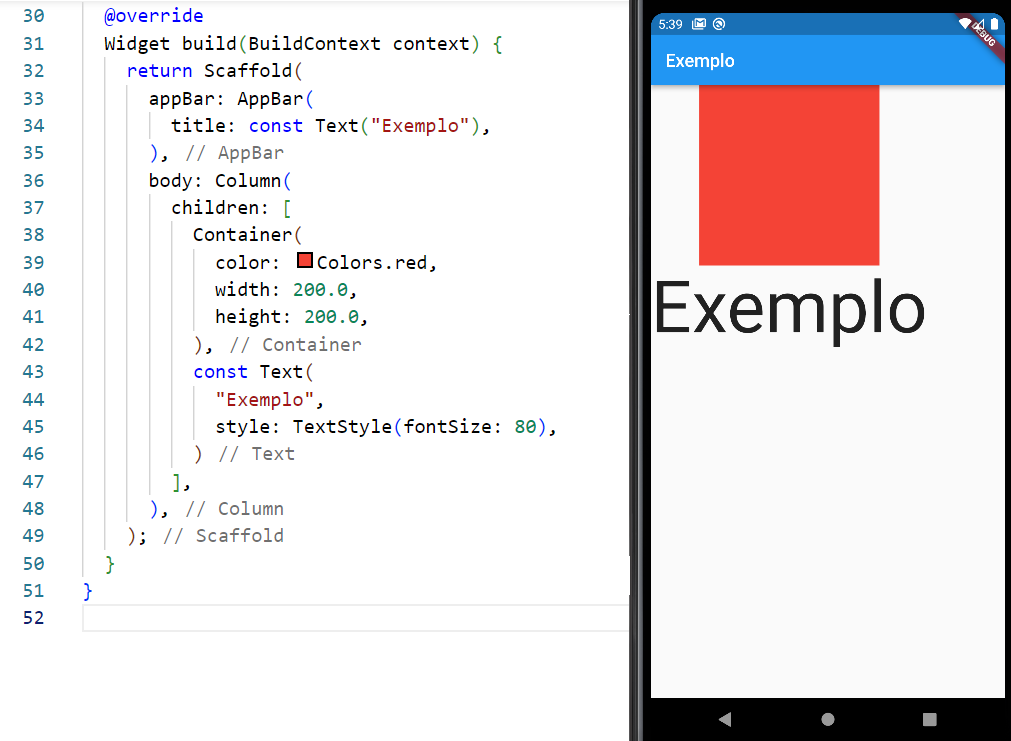
\includegraphics[width=.8\textwidth]{imagens/exemploFlutter.png}
\caption{Exemplo de Widget no Flutter}
\label{fig:widget}
\end{figure}

O Flutter engine é a parte central do Flutter que permite renderizar widgets nativos em tempo real, fornecendo uma experiência de alta fidelidade para o usuário. Ele inclui um mecanismo de layout personalizado que fornece alta performance e eficiência de memória, permitindo que o Flutter execute aplicativos móveis de alta qualidade em dispositivos com recursos limitados.


\subsection{Arquitetura} \label{sec:arq}

Arquitetura de \textit{software} refere-se ao projeto estrutural e organização de um sistema de \textit{software}, incluindo suas diferentes partes e como elas se relacionam \cite{ref_4}. A arquitetura de \textit{software} visa garantir que o sistema atenda aos requisitos de negócio e de usuário, bem como aos padrões de qualidade, desempenho, segurança e escalabilidade. 

O \textit{Back-End} é a parte do sistema que é responsável pela lógica de negócios, processamento de dados, armazenamento e gerenciamento de informações. Isso inclui o servidor, o banco de dados e o código de \textit{Back-End}, geralmente escrito em linguagens como Java, Python, Ruby ou Node.js. O \textit{Back-End} utilizado neste trabalho já se encontrava desenvolvido pelo professor da disciplina de Programação Móvel do curso de Bacharelado em Sistemas de Informação do IFBA, campus Vitória da Conquista. Foi escrito utilizando a linguagem Python, o banco de dados MySQL e Nginx como um servidor de arquivos estáticos. Ou seja, para a realização deste trabalho, não foi necessário criar o \textit{Back-End}, que foi reaproveitado da versão atual usada em sala de aula.

Já o \textit{Front-End} é a parte do sistema que é visível para o usuário, ou seja, a interface do usuário e a experiência do usuário. Isso inclui a página da web, o aplicativo móvel ou desktop, e o código de \textit{Front-End}, geralmente escrito em linguagens como HTML, CSS e JavaScript. Neste trabalho será utilizada a linguagem Dart. No escopo deste trabalho um novo \textit{Front-End} foi desenvolvido em Flutter e integrado ao \textit{Back-End} já existente.

\section{O Melhores Marcas} \label{sec:marcas}

O Melhores Marcas é a app utilizada como material didático na disciplina de Programação Móvel do curso de Bacharelado de Sistemas de Informação do IFBA, campus Vitória da Conquista. Ele apresenta uma tela de \textit{feed} (ou uma lista) que mostra produtos diferentes dispostos em cards (pequenos cartões para visualização de informações sobre os produtos).

A tela de \textit{feed} contém também um mecanismo de \textit{lazy-loading}, ou “carregamento atrasado” em português, onde apenas alguns cards são carregados para serem exibidos inicialmente e, a partir do momento o usuário chega ao fim da listagem destes, outros (cards) são carregados para serem exibidos. Dessa forma, não carregando dados que o usuário possivelmente não chegaria a listar e ver, tal mecanismo ajuda no desempenho da aplicação ao mesmo tempo que permite uma redução do consumo de banda de dados do usuário. 

Na Figura \ref{fig:feeds}, é possível observar o processo do \textit{lazy-loading}, onde a tela apresenta na interface os cards já carregados previamente. Uma fila de cards espera para que possam ser carregados posteriormente assim que o usuário chegar ao fim dos que foram previamente carregados, repetindo esse processo até que a fila (de cards) termine. Tal mecanismo se encontra presente em muitos aplicativos modernos, tais como, na listagem de imagens e vídeos do Instagram, na listagem de mensagens exibidas pelo facebook, entre outros.

\begin{figure}[ht!]
\centering
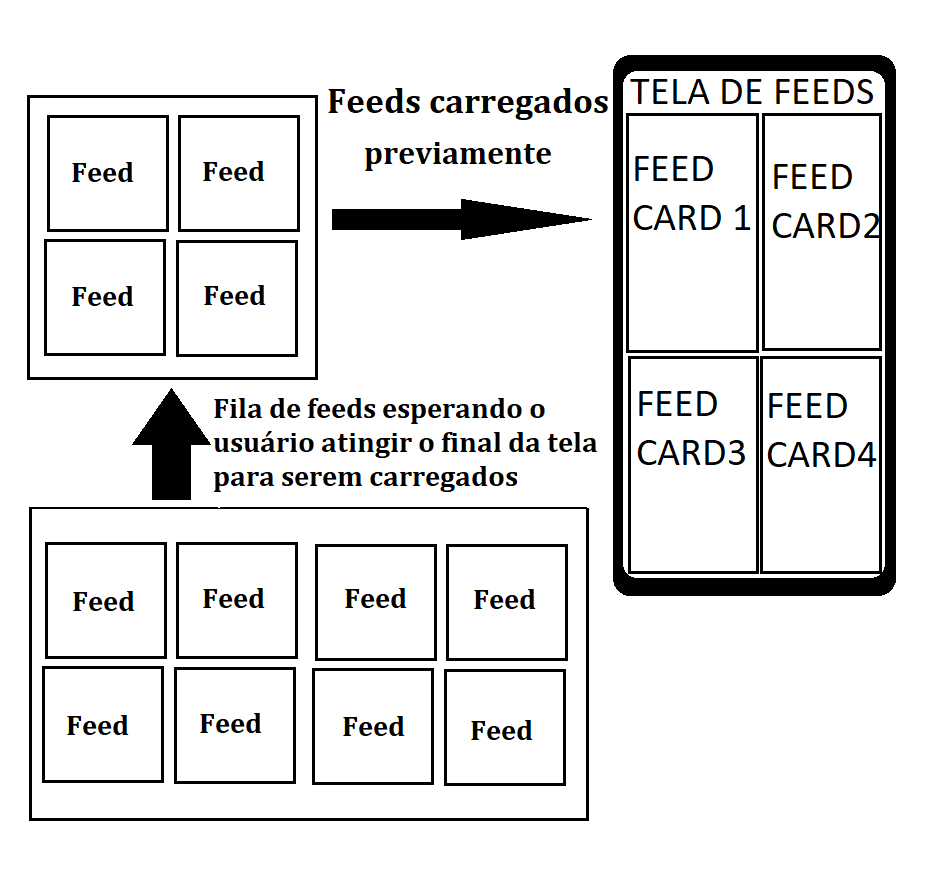
\includegraphics[width=.8\textwidth]{imagens/feeds.png}
\caption{Demonstração simples do \textit{lazy-loading}}
\label{fig:feeds}
\end{figure}

Os cards, ao serem pressionados, direcionam o usuário a uma tela de detalhes do produto, como mostra a Figura \ref{fig:telas}. Nesta tela são reapresentados os dados do produto que estão no card. Além de permitir que o usuário possa ler comentários de outras pessoas, ele pode adicionar o seu próprio comentário e curtir ("dar like") no produto. 

Atualmente, por motivos didáticos, o aplicativo, Melhores Marcas, possui duas versões. A primeira sendo apenas o \textit{Front-End}, programado utilizando JavaScript juntamente ao React-Native. Além disso, utiliza dados estáticos, armazenados em arquivos JSON local, embutido no código, simulando um acesso a dados. Já a segunda versão utiliza uma versão alterada do \textit{Front-End} com uma integração a um \textit{Back-End}, que utiliza o Python como sua linguagem de programação, o MySQL como banco de dados para os dados dos produtos e o Nginx como servidor de imagens.

\begin{figure}[ht!]
\centering
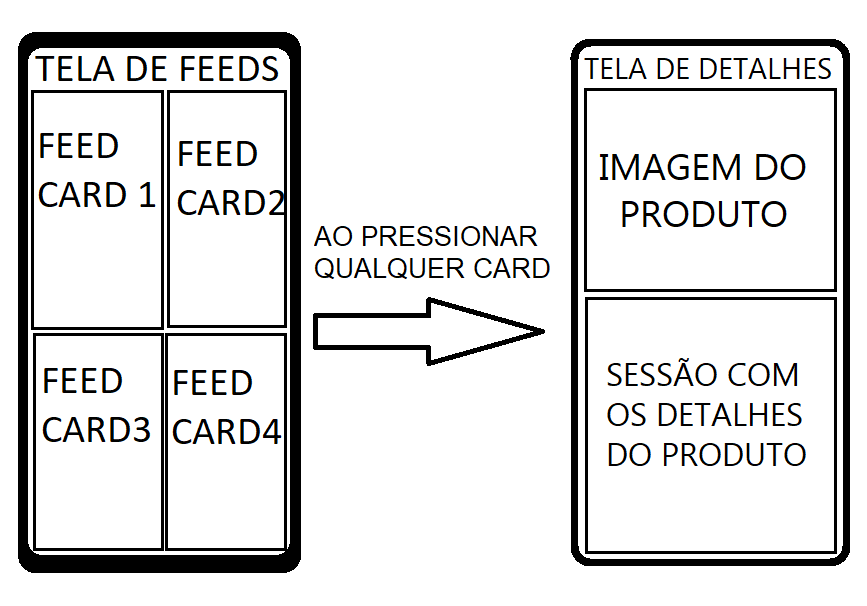
\includegraphics[width=.8\textwidth]{imagens/Navegar telas.png}
\caption{Demonstração da navegação entre telas}
\label{fig:telas}
\end{figure}

O \textit{Back-End} do Melhores Marcas é composto pelo banco de dados que contém as informações dos produtos e 3 serviços, um para o \textit{feed} dos produtos, outro para gerenciar as curtidas/likes e um terceiro para os comentários. Esses serviços coletam os dados do banco e os disponibilizam para o \textit{Front-End} através de uma API baseada em rotas http (URLs). Esse processo é ilustrado na Figura \ref{fig:backend}.

\begin{figure}[ht!]
\centering
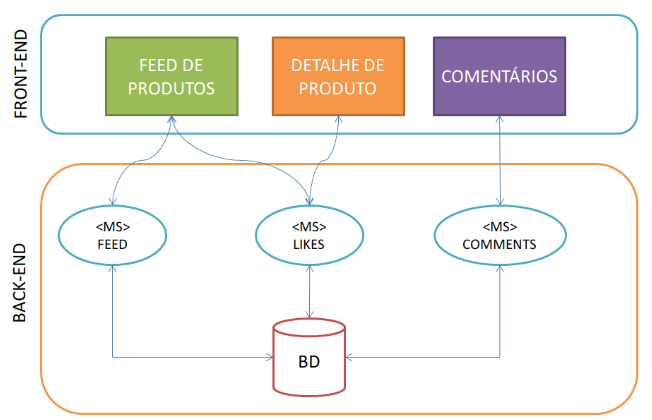
\includegraphics[width=.8\textwidth]{imagens/backend.png}
\caption{Integração \textit{Back-End} com \textit{Front-End}}
\label{fig:backend}
\end{figure}

\section{Uma versão Flutter do Melhores Marcas} \label{sec:versao}

Essa é a versão que foi implementada por esse trabalho e que buscou replicar o aplicativo existente, feito em React-Native, da maneira mais fiel possível, mas utilizando outra linguagem de programação e \textit{framework}, sendo eles o Dart e o Flutter, respectivamente. Assim como a aplicação original em React-Native, essa também se apresentará em duas versões: a primeira contando apenas com o \textit{Front-End} e a segunda com integração ao \textit{Back-End} (o mesmo \textit{Back-End} utilizado pela versão React-Native). 

As duas versões em Flutter do Melhores Marcas foram desenvolvidas durante esse trabalho e apresentam tudo que o original em React-Native tem, a listagem dos produtos em \textit{feed}, o mecanismo de \textit{lazy-loading}, o reload dos \textit{feeds}, integração com o login do Google e os cards já cumprem sua função de direcionar o usuário para tela de detalhes ao serem pressionados.

Na Figura \ref{fig:comp1}, é possível ver lado a lado a tela de \textit{feed} na versão original em React-Native (lado esquerdo) e a versão dessa mesma tela em Flutter (lado direito).

\begin{figure}[ht!]
\centering
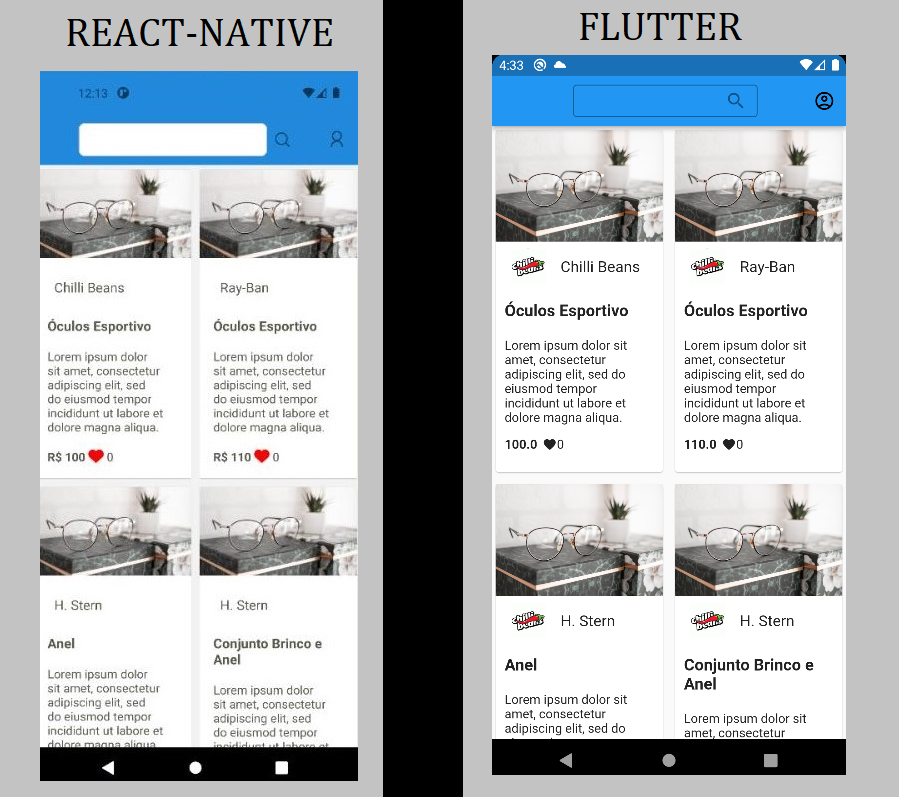
\includegraphics[width=1.0\textwidth]{imagens/compfeeds.png}
\caption{Tela de \textit{feed} de produtos reimplementada}
\label{fig:comp1}
\end{figure}

A Figura \ref{fig:comp2} apresenta um comparativo entre a tela de detalhes na versão em React-Native e a versão em Flutter. Uma grande alteração foi feitas na versão desenvolvida por esse trabalho, que foi a substituição do botão de comentário na parte superior direita por um campo, logo acima de onde são exibidos os comentários.

\begin{figure}[ht!]
\centering
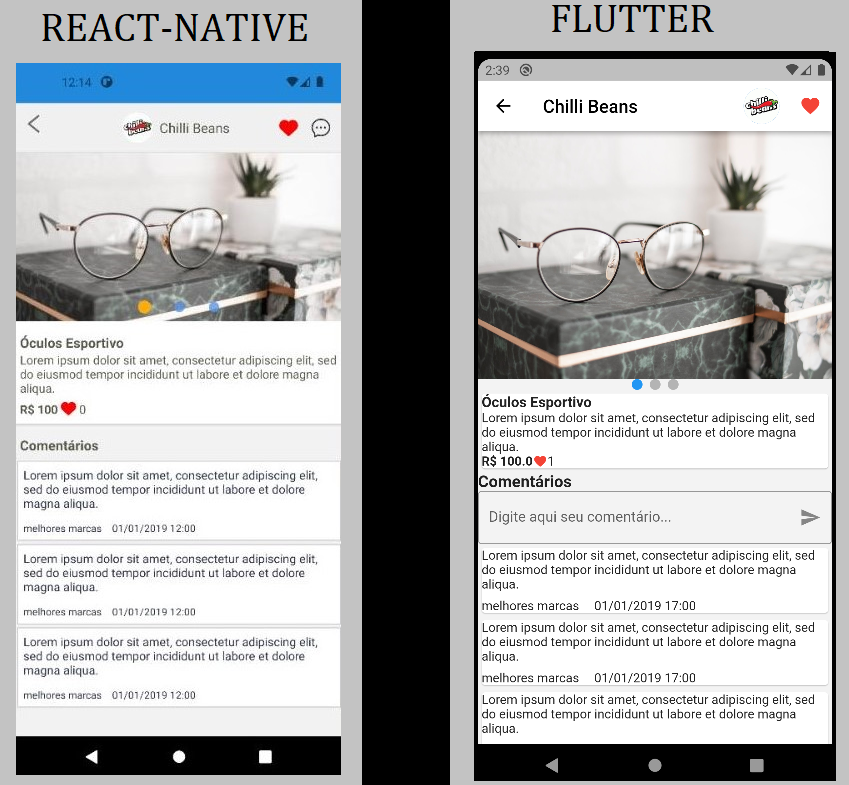
\includegraphics[width=.8\textwidth]{imagens/comparativoDetalhes2.png}
\caption{Tela de detalhes sobre produto reimplementada}
\label{fig:comp2}
\end{figure}


\section{Avaliação comparativa entre REACT-NATIVE e FLUTTER} \label{sec:aval}

Com a versão Flutter do aplicativo Melhores Marcas em mãos, foi realizado um estudo comparativo entre as duas plataformas. O estudo buscou responder algumas perguntas de pesquisa através de uma análise métrica e da experiência apreendida durante o desenvolvimento. Foram duas as perguntas de pesquisa: 

\begin{enumerate}
    \item \textbf{Pergunta de Pesquisa 1 (PP1)}: Aplicativos Móveis escritos com Flutter são mais otimizados do que se forem escritos com React-Native em termos de velocidade de execução? Uma das supostas vantagens de Flutter é que seus aplicativos executam de forma rápida, mas é necessário averiguar isto de forma comparativa; 
    \item \textbf{Pergunta de Pesquisa 2 (PP2)}: Em comparação com o React-Native, quais são os benefícios de executar as atividades de desenvolvimento de Aplicativos Móveis através da integração do Flutter com uma IDE de desenvolvimento? Uma notificação ruim constante, tanto do professor quanto dos alunos da disciplina de Programação Móvel é a dificuldade de se realizar operações básicas de codificação com o React-Native: compilação, depuração e execução. Isso se dá pela ausência de uma boa integração entre o \textit{framework} e a IDE de desenvolvimento (VSCode). O Flutter oferece algo para atenuar ou resolver este problema?
\end{enumerate}

\subsection{RESPONDENDO PP1} \label{sec:pp1}

Para responder esta pergunta de pesquisa, foi montado um ambiente de teste em uma máquina DELL, com processador i7 da oitava geração, com 16 gigabytes de memória e ambiente operacional Linux Mint.

Foram realizados 5 testes com cada versão (React-Native x Flutter). Os testes consistiram em modificar o código dos aplicativos para que fosse contabilizado o tempo desde que a tela de \textit{feed} de produtos é exibida até o momento que os primeiros produtos (ou página) do \textit{feed} é construído e mostrado.

A Figura \ref{fig:graficos} apresenta os resultados dos testes a partir de gráficos comparativos, elencando cada teste lado a lado. 

\begin{figure}[ht!]
\centering
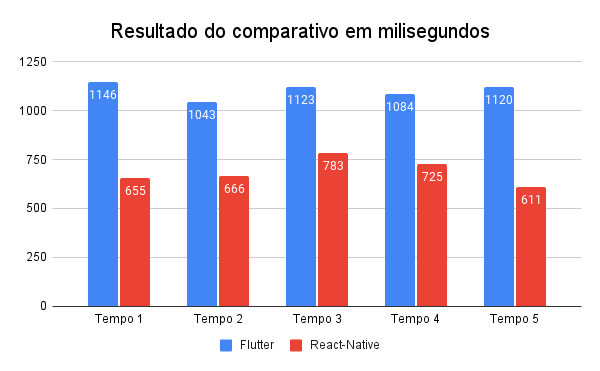
\includegraphics[width=.8\textwidth]{imagens/grafic.png}
\caption{Gráfico comparativo dos tempos de cada versão}
\label{fig:graficos}
\end{figure}

Como pode ser observado, o React-Native teve grande vantagem nos seus tempos, chegando até a realizar o carregamento dos \textit{feeds} em aproximadamente 54\% do tempo do Flutter (como mostra o resultado do Tempo 5). O uso de uma versão de depuração da aplicação em Flutter pode ser a causa dessa discrepância entre os resultados dos testes. A utilização de uma versão de \textit{release} das aplicações resultaria em tempos mais parelhos entre os \textit{frameworks}.

\subsection{RESPONDENDO PP2} \label{sec:pp2}

A integração do Flutter com o VSCode (IDE utilizada durante o trabalho) traz bastante benefícios na hora de depurar ("debuggar") o código, tornando mais fácil encontrar erros na construção do app. Essa ajuda vem principalmente a partir do console que retorna os problemas encontrados na execução do código. O plugin oficial de integração entre o Flutter e o VSCode permite que o programador interrompa momentaneamente a execução e prossiga com a execução do código à medida que analisa diferentes cenários de desenvolvimento e resolução de erros. Tais funcionalidades estão destacadas na Figura \ref{fig:debug}.

\begin{figure}[ht!]
\centering
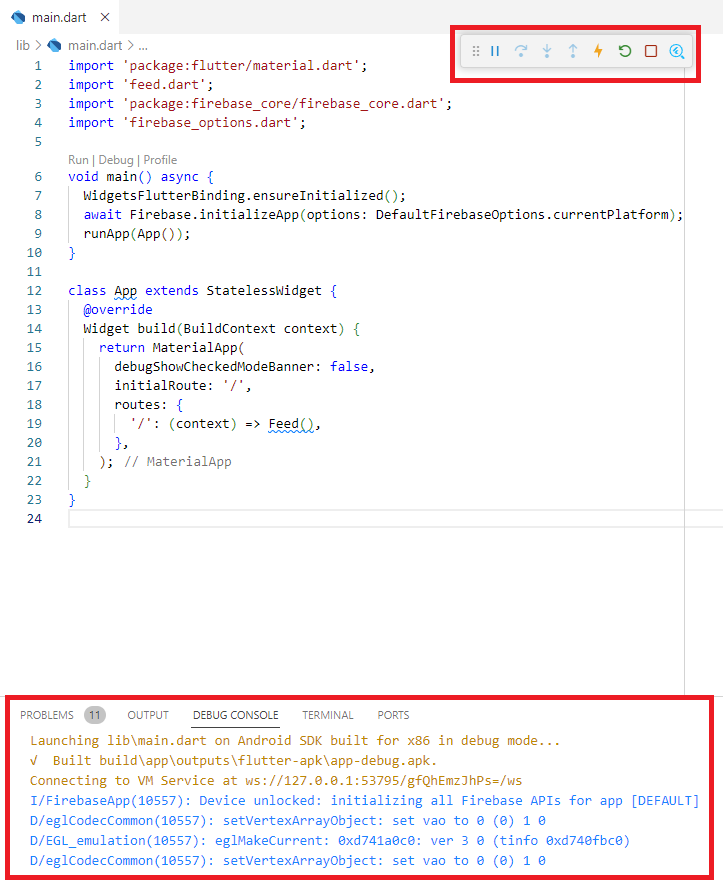
\includegraphics[width=.8\textwidth]{imagens/debugFlutter.png}
\caption{O console e o “controle” em destaque}
\label{fig:debug}
\end{figure}

Em contraste com a facilidade que apresenta o Flutter, a depuração do React-Native não ocorre de forma tão direta, pois depende do Chrome Debugger para funcionar, sendo mais limitada, como aponta Nathan Balogun \cite{ref_11}. Ele comenta também que para ajudar com as limitações, algumas ferramentas de outra linguagem de programação (java, por exemplo) podem ser utilizadas.

\section{CONCLUSÕES} \label{sec:conc}   

Esse trabalho visou entregar uma nova do versão em Flutter do app Melhores Marcas, utilizado na disciplina de Programação Móvel do curso de BSI do IFBA, campus Vitória da Conquista. Seguindo essa necessidade, surgiu também uma motivação para comparar esses dois \textit{frameworks}. A partir disso, e com o aplicativo pronto foram realizadas as comparações tendo como base a duas perguntas de pesquisa expostas na Seção \ref{sec:aval}.

Um desafio enfrentado foi “traduzir” um aplicativo construído em uma linguagem e \textit{framework} para outro. Tal tarefa requer um estudo dos componentes que a app original usava, para que fossem encontrados os correspondentes em Flutter. Antes de iniciar o trabalho, o autor principal não apresentava um grande conhecimento do Flutter, então aprender a linguagem durante a construção do app acabou representando um desafio particular, mas que foi superado. 

Esse trabalho proporcionou algumas descobertas interessantes. Por exemplo, em relação aos resultados da segunda Pergunta de Pesquisa (Seção \ref{sec:pp1}), em como o React-Native acabou se sobressaindo em comparação com o Flutter em relação ao seu desempenho. Vale ressaltar, todavia, que a versão do aplicativo Flutter utilizado foi a de depuração. Os resultados seriam diferentes se a comparação fosse realizada sobre versões finais, de \textit{release}, dos \textit{softwares}.

A facilidade de utilizar e depurar o Flutter utilizando uma IDE como o VSCode se provou relevante durante o desenvolvimento da aplicação, ajudando em diversos momentos a encontrar e corrigir os problemas do código com bastante facilidade. Em comparação com o React-Native, o autor deste trabalho entende que isto é bastante vantajoso, já que este é um recurso que, quando falta, dificulta o aprendizado e uso deste tipo de tecnologia, algo percebido durante as aulas da disciplina de Programação Móvel do curso de Bacharelado de Sistemas de Informação do IFBA, campus Vitória da Conquista.

\subsection{TRABALHO FUTUROS} \label{sec:trabalhos}

A partir do que foi feito neste trabalho, existem algumas outras possibilidades para se aprofundar mais no tema. Uma delas seria a utilização de um aplicação mais robusta e com mais telas e funcionalidades. Com uma aplicação maior seria possível verificar mais diferenças entre os 2 \textit{frameworks}. Tal cenário também pode favorecer as comparações de desempenho entre Flutter e React-Native, pois explorando mais funcionalidades pode ser possível encontrar alguma(s) onde um \textit{framework} acaba se sobressaindo. 

Como apontado na resposta da Pergunta de Pesquisa 1, os resultados que esse trabalho apresentou se deram apenas com uma versão de depuração da aplicação em Flutter. Um possível trabalho futuro seria realizar os mesmos testes mas com uma versão de \textit{release} dos apps utilizados.

Outro trabalho que pode ser realizado é buscar outros \textit{frameworks} para serem adicionados ao comparativo. Por exemplo, utilizar o Kotlin, que é outra tecnologia bastante empregada na construção de \textit{softwares} móveis.

Por fim, uma última possibilidade é buscar outros casos de aplicativos desenvolvidos utilizando React-Native ou Flutter, e, a partir disso, contactar suas empresas e/ou os desenvolvedores para entender o que os fizeram escolher o \textit{framework} utilizado e, assim, encontrar quais as vantagens que acabaram se tornando atrativos na prática.

\subsection{CONTRIBUIÇÕES} \label{sec:contribuicoes}

Esse trabalho deixa algumas contribuições. A primeira delas é o tema principal abordado, as diferenças entre Flutter e React-Native, deixando um estudo comparativo para ajudar quem estiver em dúvida sobre qual escolher. 

O código fonte de ambas as versões desenvolvidas em Flutter estão disponíveis e elencadas na Tabela \ref{tab:versoes}. A tabela apresenta links que direcionam ao repositório de cada versão da aplicação durante seu desenvolvimento. 

\begin{table}[ht!]
    \centering
    \begin{tabular}{|c|c|c|}\hline
         Versão & Tag & Link \\\hline
         Apenas \textit{Back-End} & v0.1 & https://x.gd/v3OLG \\\hline
         Apenas \textit{Back-End} & v0.2 & https://x.gd/0lIqL \\\hline
         Apenas \textit{Back-End} & v0.3 & https://x.gd/lggo7 \\\hline
         Apenas \textit{Back-End} & v0.4 & https://x.gd/wynJt \\\hline
         Apenas \textit{Back-End} & v0.5 & https://x.gd/uK1hX \\\hline
         Apenas \textit{Back-End} & Final & https://x.gd/x8YBG \\\hline
         \textit{Front-End} integrado & Final & https://x.gd/IjM5k \\\hline
    \end{tabular}
    \caption{Versões Flutter do Aplicativo Melhores Marcas}
    \label{tab:versoes}
\end{table}

Para finalizar, a contribuição principal deste trabalho é a utilização do app desenvolvido durante a disciplina de Programação Móvel no semestre 2023.2. Enquanto essa disciplina tiver o Flutter como  \textit{framework} utilizado nas aulas para lecionar o conteúdo, a aplicação continuará a ser utilizada durante as aulas, possibilitando o ensino de programação móvel para muitos alunos em momentos atuais e futuros.

\bibliographystyle{sbc}
\bibliography{bibliografia}

\newpage

\noindent\textbf{Apêndice}

Os conceitos adquiridos durante o curso de Bacharelado em Sistemas de Informação (BSI) pelo Instituto Federal de Educação, Ciência e Tecnologia da Bahia contribuíram para a construção do projeto, desde o levantamento teórico até a aplicação prática.

A Figura \ref{fig:disciplinas} demonstra todas as disciplinas que contemplam a ementa do curso de BSI e que se relacionam de forma direta e indireta com a elaboração do projeto.

\begin{figure}[ht!]
\centering
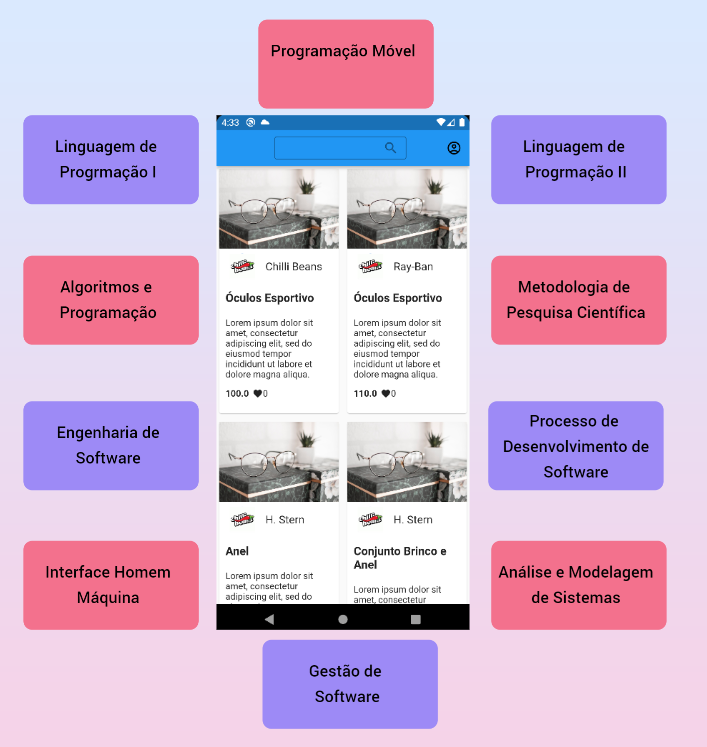
\includegraphics[width=1.0\textwidth]{imagens/disciplinas.png}
\caption{Disciplinas que contribuíram na elaboração deste trabalho}
\label{fig:disciplinas}
\end{figure}

\end{document}
